\documentclass[12pt]{article}
\usepackage[backend=biber]{biblatex}
\addbibresource{ProjectProp.bib}

\usepackage{graphicx} %intersting images
\usepackage{float} %for placement of images
\usepackage{lipsum} %fill
\usepackage{tocloft} %for dots on table of contents
\renewcommand{\cftsecleader}{\cftdotfill{\cftdotsep}}


%\renewcommand{\abstractname}{Thesis}

\title{\textbf{Senior Capstone Project - Charge Pump}}
\author{Derek Brissey \& John Clapham\\ \textit{Advisor: Dr. Brian Huggins \& Dr. Prasad Shastry}\\ Capstone Project}
\date{Nov 13, 2019}

\begin{document}

\begin{titlepage}
	\centering{
\includegraphics[scale=0.7]{ProjectPropFigure/BUlogo.jpg}\\
	\vspace{3em}
	\bfseries{\large{Department of Electrical and Computer Engineering}}\\
	\vspace{2em}
	\bfseries{\large{Senior Capstone Project}}\\
	\vspace{2em}
	\bfseries{\Large{Charge Pump}}\\
	\vspace{2em}
	\bfseries{\large{Authors: Derek Brissey \& John Clapham}}\\
	\textit{\large{Advisors: Dr. Brian Huggins \& Dr. Prasad Shastry}}\\
	\vspace{2em}
	\today
	}
\end{titlepage}

	\pagenumbering{roman}

	\begin{abstract}
Radio frequency (RF) power sipping devices can be a useful alternative for low power applications such as periodic sensor measurements. Many papers have been published with different radio frequency to direct current (RF-DC) architectures. A passive charge pump topology using Schottky Diodes and capacitors to step up the voltage to a usable steady state can eventually be released as direct current. This capstone project will include research and simulation, design, and eventually populating a printed circuit board (PCB) with specified components for testing. Three main topologies for the charge pump will be investigated to help determine the best choice considering: optimum number of stages, the capacitor values, and the type of switch to be used.
	\end{abstract}
	
	\newpage
	\tableofcontents
	\newpage
	
	\pagenumbering{arabic}
	
	\section{Introduction}
	Electromagnetic signals that typically oscillate in the range of 3kHz to 300GHz are known as Radio Frequency~(RF) waves. The low power signal that is left over from RF transmissions in the air could be absorbed and used to supply power to a device; this process is known as energy harvesting. It is normally difficult to siphon off enough energy from these RF signals to be usable due to their low input power to energy harvesters. A charge pump is a circuit typically used to change the output voltage of a DC device, however, research suggests a charge pump could be used as an energy harvester to raise a low power high frequency RF signal to a usable steady state DC voltage level. Charge pumps have several different topologies but typically act as a multiplier of some sort. Many attempts to optimize the selection of components have been made. A formula for selecting capacitor values and number of stages in order to optimize the performance of the charge pump is the goal of this project.

	\section{Project Description}
	A charge pump is a DC-DC converter that uses capacitors to store and release charges to raise or lower the output voltage of a device. If a charge pump could be modified to instead use the input of a high frequency AC signal to charge a series of capacitors and eventually output a DC signal, it could be used as a wireless energy harvester. There are many applications for implementing the charge pump as a passive power sipping device that absorbs high frequency energy signals (from sources such as cell phone towers, radio towers, wireless transmitters, etc.) and outputs a DC signal. Multiple papers exist documenting the progress that has been made in radio frequency to direct current~(RF-DC) devices, however, further investigation is needed for improving the efficiency of power conversion, as well as possible circuit topologies, and device implementations. Due to the low turn on voltage of Schottky diodes, they tend to be a popular choice in charge pump designs. Other switches have been used such as MOS transistors, and will be investigated during the research stage as well. Impedance matching design will also be considered to deliver the highest output power possible. Power efficiencies will need to be measured to determine an understanding of the most effective circuit topology.
	
	\section{Review of Design}
	Charge pumps are used to passively siphon off RF signals and produce a DC output. The DC output is obtained by the capacitors cyclically charging and discharging depending on the state of a few diodes. Several characteristics must be considered when designing a charge pump circuit. The minimum voltage amplitude determined from the load current and output voltage is referred to as the sensitivity of the circuit. The sensitivity is one of the more important metrics to consider when designing the charge pump because it indicates the minimum power necessary at the input of the charge pump that will supply a DC voltage to the periodic load. Two other important metrics to consider are the power conversion efficiency~(PCE) and the voltage conversion efficiency~(VCE) given in equations 1.0 and 1.1~(pages 4 and 5). Balance between sensitivity and PCE must be made because minimizing power loss improves PCE, but higher sensitivity may degrade the PCE.  Power Efficiency~(PE) is a metric regarding power delivered to the load to power supplied at the receiver. PE and PCE can be the same if there is no impedance matching or components before the charge pump.  If impedance matching is used Power Transfer Efficiency~(PTE) which is the amount of AC power at the receiver to the power at the transmitter inductor. The sensitivity, PCE, VCE, and PE are all metrics to be considered when choosing the topology used. Dickson multiplier topology is the most common topology used. Cross-coupled multiplier topology is another option used to reduce both reverse leakage and the on-resistance of transistors.
	
	\section{Project Plan}
	The purpose of this project is to have a functioning RF power sipping device on a printed circuit board~(PCB). The project will result in providing research for more effective topologies and components used to produce a low voltage DC output. The three main stages of the project will include research, simulation, design, and implementation on a PCB. While the idea is to convert RF frequencies~(greater than 500MHz) to DC, experimentally we will use less than 1~MHz to get an accurate time domain response. After implementing to a PCB tests will run up to the MHz range. The functional requirements for the project are listed below:\\
	
\noindent{Functional Requirements}
\begin{itemize}
	\item Convert RF signal input to a DC signal output
	\item Maximize steady state DC output
	\item Explore different charge pump designs
	\item Design and print circuit board for testing purposes
\end{itemize}
	
	\subsection{Research}
	Research papers exploring different power sipping devices that include block diagrams, functional designs, and power efficiency equations have been provided. A research paper titled ``Power Management in Wireless Power-Sipping Devices: A Survey,” by Ulkuhan Guler and Maysam Ghovanloo \cite{Guler}, provides a good starting point for an understanding of the task at hand. The paper will be used as a basis for simulation of different charge pump topologies. Other research papers that will prove useful to the development of the RF-DC charge pump have been listed in the \textit{Bibliography} section on page~\pageref{bibliography}.\\
	
	\noindent “Power Management in Wireless Power-Sipping Devices: A Survey,” explains the different types of devices that can be used to construct a charge pump. The three main topologies that exist are the Greinacher Multiplier, the Dickson Multiplier, and the Cross-Coupled Multiplier. Depending on the topology that is being constructed the components can change to increase the Power Conversion Efficiency~(PCE). PCE is the ratio of DC power delivered to the load, to the AC power delivered to the input. The equation is given as follows:\footnote{Detailed explanation of equation 1 can be found in \cite{Guler}}
	
\begin{equation}
PCE = \frac{P_{Out}}{P_{In}} = \frac{P_{Out}}{P_{Out} + P_{In}}\label{eq:PCE}
\end{equation}
\vspace{1em}
\\
The voltage conversion efficiency (VCE) is the ratio between the peak voltage available at the input of the device and the DC voltage available at the output. The equation is given as follows:\footnote{Detailed explanation of equation 1 can be found in \cite{Guler}}

\begin{equation}
VCE = \frac{DC Output Voltage}{RF Peak Voltage} = \frac{V_{Out}}{V_{P}}\label{eq:VCE}
\end{equation}
\\
	The PCE and VCE equations can be used to compare the efficiency variability in the different designs that will be simulated. PCE and VCE can be optimized by carefully selecting the parts used in the charge pump. Three of the main switching devices used are Schottky diodes, diode-connected transistors, and ultra-low power diodes. Deciding which of these devices to use is based on factors such as the reverse leakage, forward loss, and availability in standard CMOS processes. Lower levels of reverse leakage improve the PCE of the device which is a big deciding factor in choosing switching devices.
	
	\subsection{Design/Simulation}
	Simulations of the charge pump will be done using ORCAD PSpice. The simulation process will start by designing a single stage charge pump in PSpice. The starting design will be based on the standard Dickson charge pump with 1uF capacitors and Schottky diodes. The input signal will start at 1KHz with the results being gathered in the time domain.\\
	
	\noindent After analysis of the one stage charge pump response, various topologies will be created for analysis consisting of different numbers of stages, and different capacitor values. Stages will continue to be added until a three stage charge pump is created. The time domain response will be recorded from all three designs, and then be compared. The most effective design with the best PCE and VCE values~(equations~\ref{eq:PCE}~and~\ref{eq:VCE} on pages~\pageref{eq:PCE} and~\pageref{eq:VCE}) will be selected from the three designs. After selecting the design the values of the capacitors will be varied. Simulations will be run in the time domain to analyze the effect of varying values. Next, different topologies will be explored to see if the design can be further improved. A high level block diagram of the energy harvester to be designed is shown in Figure~\ref{fig:HighLevel} on page~\pageref{fig:HighLevel}.\\
	
\vspace{0.5em}
\begin{figure}[H]
\centering{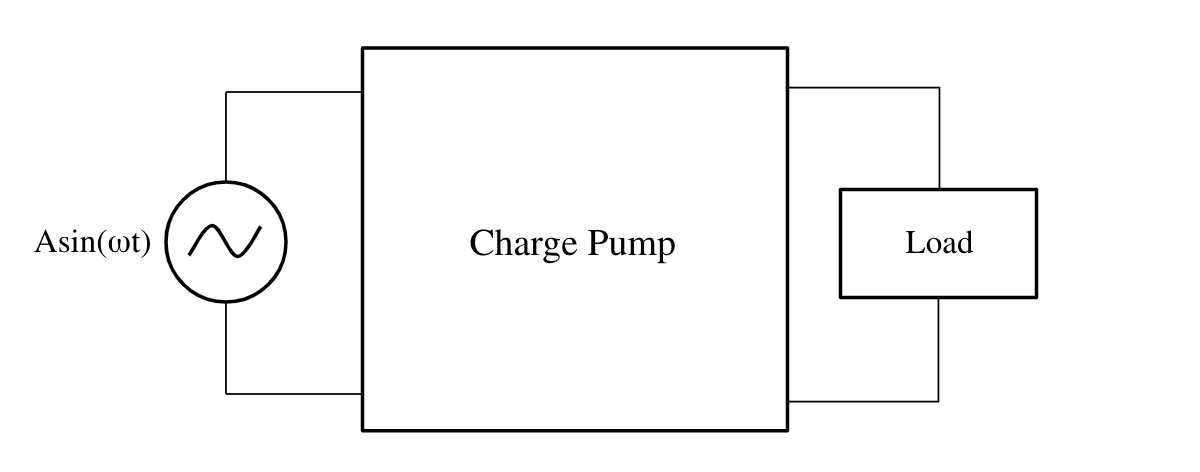
\includegraphics[scale=0.5]{ProjectPropFigure/HighLevelBlock.png}}
\caption{High Level Block Diagram}
\label{fig:HighLevel}
\end{figure}

\noindent The high level block diagram shows the overarching design of the energy harvester. Only the charge pump, a sinusoidal input, and a load are necessary to represent the system. The underlying charge pump block can be varied through different suggested topologies. Figure~\ref{fig:DicksonCP}  on page~\pageref{fig:DicksonCP} shows the circuit topology that will be used for a majority of the simulation and design stages.

\vspace{0.5em}
\begin{figure}[H]
\centering{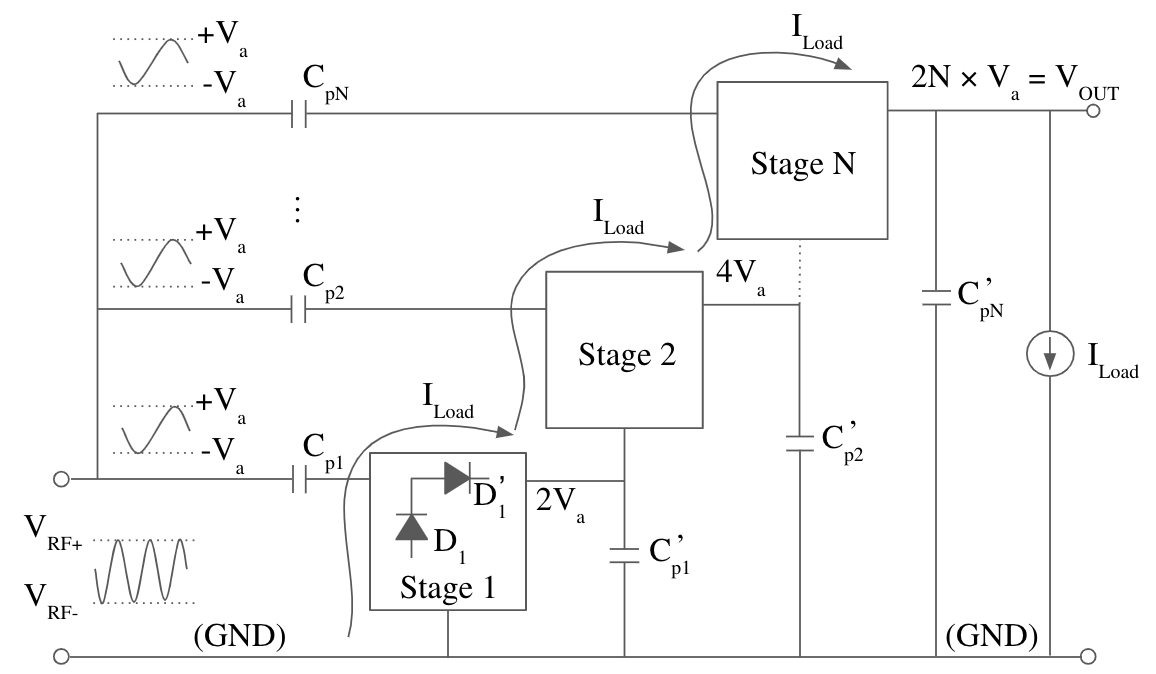
\includegraphics[scale=0.5]{ProjectPropFigure/DicksonBlock.png}}
\caption{Dickson Charge Pump Block \cite{Guler}}
\label{fig:DicksonCP}
\end{figure}

	\subsection{Implementation}
	Once the simulations have been completed, a board design can be created for testing purposes. Prototyping will be done using breadboards and components in the lab. Once verified, a board will be designed and sent to an outside board printing company. The PCB will then be populated with components selected to our specification for testing purposes.
	
	\subsection{Inputs and Outputs}
	
\noindent{Input}
	\begin{itemize}
		\item High frequency signal (from signal generator)
	\end{itemize}
\noindent{Output}
	\begin{itemize}
		\item DC signal
		\item Time domain response graph
	\end{itemize}
	
	\section{Analysis and Simulation}
	
	\subsection{Current Progress}
	Simulations of a two stage Dickson charge pump with an input amplitude of 1V with a frequency of 1kHz. The circuit was constructed using the PSpice program. Components were selected to best reflect the physical components available to build a prototype. Standard 1uF capacitors and BAT68 diodes were selected to emulate the standard capacitor values and Schottky diodes provided to build the circuit. Figure~\ref{fig:2SCP NSR} shows the layout of the designed charge pump. Time domain responses were plotted showing the voltage stepping up to a steady state. The results were recorded for 300 microseconds. Figures~\ref{fig:2SCP NSR} and~\ref{fig:2SCP NSR Out} on pages~\pageref{fig:2SCP NSR} and~\pageref{fig:2SCP NSR Out}  show the layout of the designed charge pump and the output voltage at the load resistor respectively.
	
\vspace{0.5em}
\begin{figure}[H]
\centering{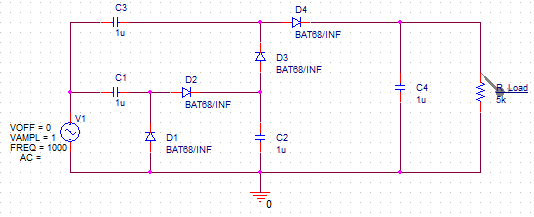
\includegraphics[scale=0.7]{ProjectPropFigure/CP1p1000f.png}}
\caption{2-Stage Charge Pump (No Source Resistance)}
\label{fig:2SCP NSR}
\end{figure}

\vspace{0.5em}
\begin{figure}[H]
\centering{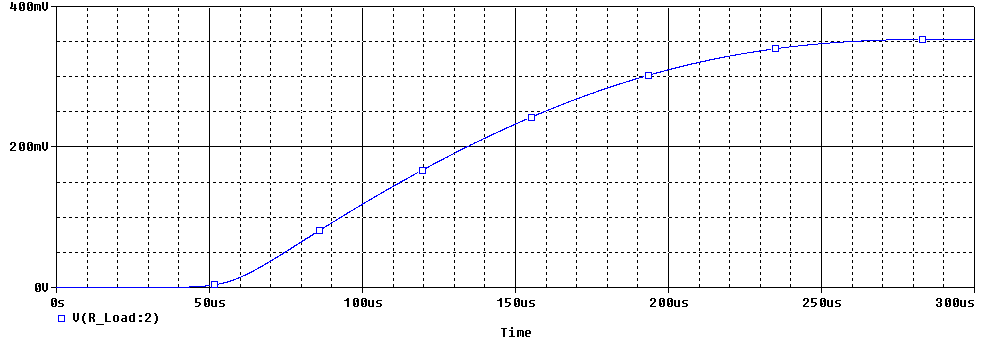
\includegraphics[scale=0.45]{ProjectPropFigure/CPsim300us.png}}
\caption{2-Stage Charge Pump Output Voltage (No Source Resistance)}
\label{fig:2SCP NSR Out}
\end{figure}

	\noindent Analysis of the Bat68 Diode turn on voltage was simulated in Pspice as well. A DC sweep has been performed with a step voltage of 1mV in order to compare the forward voltage listed on the data sheet. The simulation design is shown in Figure~\ref{fig:Bat68Analysis} on page~\pageref{fig:Bat68Analysis} with the output of the DC sweep shown in Figure~\ref{fig:Bat68Knee} on page~\pageref{fig:Bat68Knee}. The simulation results compare to the data sheet values of the Bat68's typical forward voltage of 318mV. These simulations are likely to be repeated to determine the diode with the lowest turn on voltage within a reasonable price range.

\vspace{0.5em}
\begin{figure}[H]
\centering{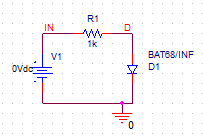
\includegraphics[scale=0.7]{ProjectPropFigure/Bat68.png}}
\caption{Bat68 Diode Analysis Setup}
\label{fig:Bat68Analysis}
\end{figure}

\vspace{0.5em}
\begin{figure}[H]
\centering{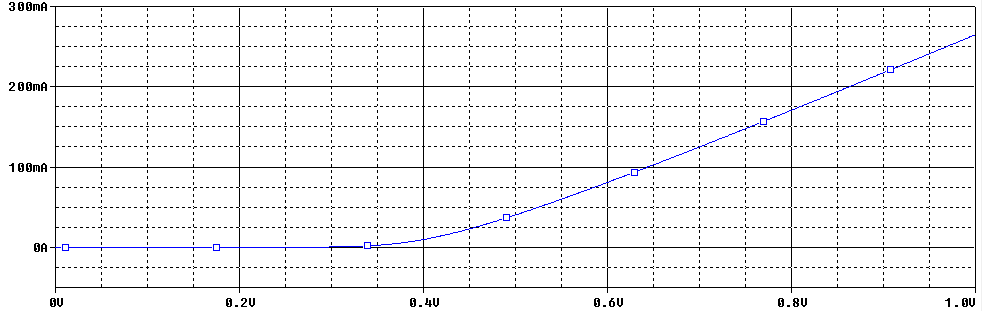
\includegraphics[scale=0.45]{ProjectPropFigure/Bat68Knee.png}}
\caption{Bat68 Diode Knee Voltage}
\label{fig:Bat68Knee}
\end{figure}

\noindent A 50 Ohm resistor was added as a source resistance to reflect the response of a practical circuit~(see~Figure~\ref{fig:2SCP SR}). The time domain responses of the voltage was taken of the circuit and compared to the response of the circuit without the source resistance. The Simulation was run for 350 microseconds to account for the longer steady state rise time~(see~Figure~\ref{fig:2SCP SR Out}) compared to simulation shown in Figure~\ref{fig:2SCP NSR Out}.\\

\vspace{0.5em}
\begin{figure}[H]
\centering{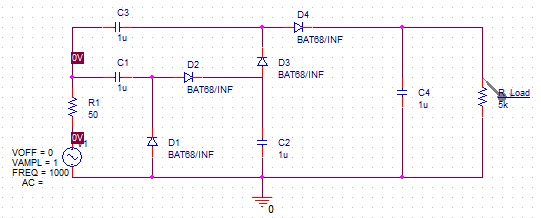
\includegraphics[scale=0.7]{ProjectPropFigure/CPWSR.png}}
\caption{2-Stage Charge Pump (With Source Resistance)}
\label{fig:2SCP SR}
\end{figure}

\vspace{0.5em}
\begin{figure}[H]
\centering{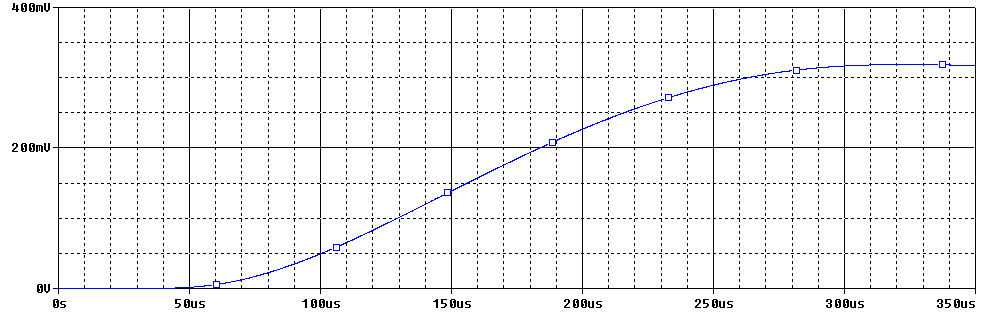
\includegraphics[scale=0.45]{ProjectPropFigure/CPsimWSR.png}}
\caption{2-Stage Charge Pump Output Voltage (With Source Resistance)}
\label{fig:2SCP SR Out}
\end{figure}

\noindent Physical circuits of the designs were constructed to measure the response in real time. In physical circuit tests ceramic capacitors and Schottky diodes 1N5817 were provided by the labs and used. The input signal was supplied by a function generator.

	\subsection{Future Plans}
	More simulations must be performed in an effort to optimize the construction of the charge pump. Tests will be performed by varying the different number of levels in the charge pump versus the value of the capacitors to verify which causes a charge pump of charge up faster. Ideally the simulations can be performed and finished over winter break and January. Circuits will be built in the labs in February and March. An attempt to find a correlation or formulate some equation that will optimize the values of capacitors and number of levels for a charge pump will be made using the results of the simulations and physical circuit tests. By the end of March to mid April a circuit board prototype will be made. Parts to construct a PCB will need to be ordered at a later date when a method for optimization is formulated.
	
	\section{Conclusion}
	Future uses for RF-DC power sipping devices include any low power applications such as period measurement systems, medical sensors, space and aerospace applications, etc. The experience gained from this capstone project will transfer into hardware design and RF design. After designing and implementing to a physical circuit board a better understanding of the design process will be an important outcome. The hope is to have a published research paper at the end of the project as well as added experience.
	
	\newpage\label{bibliography}
	\nocite{*}
	\printbibliography
	
\end{document}